\documentclass[12pt]{article}
\usepackage{graphicx} %插入图片的宏包
\usepackage{float} %设置图片浮动位置的宏包
\usepackage{subfigure} %插入多图时用子图显示的宏包
\usepackage{amsmath,amssymb}
\usepackage{hyperref}
\usepackage[utf8]{inputenc}
\usepackage{geometry}
\usepackage{booktabs}
\geometry{a4paper, margin=1in}
\usepackage{cite}

\title{ZheDa DataSet in China}
\author{Name1, Name2, Name3}
\date{\today}

\begin{document}
\maketitle

\begin{abstract}
    
\end{abstract}

\section*{Background \& Summary}

The stability and operational efficiency of power systems are crucial for modern energy infrastructure,
especially in the context of large-scale renewable energy integration and the continuous development of smart grid technologies.
Understanding the dynamic behavior of power systems, including interactions between different types of nodes, is essential for grid optimization,
stability analysis, and operational scheduling. However, publicly available datasets that comprehensively reflect the evolving topology and electrical
characteristics of power networks over time remain limited. To address this gap, we have constructed a time-series dataset that records the topological
relationships and electrical properties of power system nodes, supporting research in power flow analysis, anomaly detection, and grid resilience assessment.  

This dataset has the following key characteristics:

\begin{itemize}
    \item \textbf{\small Topological Structure Modeling}: The \texttt{edges} array records the connections between power system nodes, providing a clear representation of the grid topology. This facilitates complex network analysis, fault propagation studies, and network optimization.  
    \item \textbf{\small Time-Series Electrical Characteristics}: The \texttt{H} matrix contains electrical parameters (e.g., voltage, current, power) for each node at different time points, supporting load analysis, power flow calculations, and time-series studies.  
    \item \textbf{\small Node Function Classification}: Three types of nodes are identified within the dataset:
    \begin{itemize}
        \item \textbf{\small PQ Nodes (Load Nodes)}: Nodes with both active power (P) and reactive power (Q) demands, which are essential for studying power distribution and dynamic load variations.  
        \item \textbf{\small PV Nodes (Generation Nodes)}: Nodes that provide active power output while maintaining a constant voltage, useful for analyzing generator operations and optimization strategies.  
        \item \textbf{\small Vt Nodes (Voltage-Controlled Nodes)}: Typically representing critical substations or power plants responsible for voltage stability, these nodes are valuable for studying grid regulation and control strategies.  
    \end{itemize}
    \item \textbf{\small Time-Series Weather Data Integration}: The dataset incorporates synchronized local weather measurements (e.g., temperature, humidity, wind speed), allowing users to investigate the influence of environmental conditions on grid behavior. This multimodal temporal data supports weather-aware forecasting, renewable integration studies, and climate resilience analysis.
    \item \textbf{\small Wide Applicability}: The dataset can be used in machine learning, deep learning, optimization algorithm testing, power grid fault prediction, power quality analysis, and smart grid control strategy research.  
\end{itemize}

The time-series nature of this dataset makes it suitable for a wide range of research applications,
including machine learning-based power system forecasting, stability assessment, and anomaly detection.
Additionally, it serves as a benchmark for optimization and control algorithm testing, contributing to the development of intelligent scheduling methods.
Unlike traditional static datasets, which typically provide only snapshots of power system states at specific moments, this dataset captures the dynamic evolution of
the grid, allowing researchers to analyze both long-term trends and short-term fluctuations. The improved temporal resolution enhances its applicability to real-world
power system analysis.  

Several datasets, such as IEEE test systems and open-source grid models, have been widely used in power system research. 
However, these datasets primarily focus on steady-state analysis and lack representations of dynamic system behavior. Additionally, 
while frameworks like MATPOWER provide computational tools for power flow analysis, they do not inherently include real-world time-series data for model validation.
 In contrast, our dataset fills this gap by offering structured time-series data, expanding the possibilities for computational experiments and analytical studies.  

This dataset holds significant reuse potential across multiple domains:

\begin{itemize}
    \item \textbf{\small Power Grid Stability and Security Analysis}: Supports the assessment of grid operational states and stability under varying load conditions and fault scenarios.  
    \item \textbf{\small Smart Grid Optimization and Scheduling}: Enables research on real-time grid optimization and scheduling, improving energy efficiency and reducing operational costs.  
    \item \textbf{\small Data-Driven Predictive Models}: Suitable for training and validating machine learning and deep learning models for tasks such as load forecasting and anomaly detection.  
    \item \textbf{\small Interdisciplinary Research}: Can be integrated with economic and market factors to study the financial impact of grid anomalies and optimize energy management strategies for economic benefits.  
\end{itemize}

Overall, this dataset provides a comprehensive, high-resolution representation of power system node interactions,
creating new research opportunities in grid modeling, machine learning applications, and energy system optimization.
By making this dataset publicly available, we aim to promote reproducible research and accelerate advancements in power system management and analysis.

\section*{Methods}
\subsection*{Data collection}
% 数据采集内容

The data is collected from the power grid of a certain area in eastern China by the D5000 system of the State Grid Corporation of China.
Data collection is primarily implemented through various sensor devices. 
After preliminary local processing, the collected data is transmitted to the system for comprehensive analysis and processing via communication networks. Typically, the data acquisition and communication subsystem in the system consists of routers, data acquisition communication servers, and serial communication devices. The normal functioning of these related equipment requires two or more application servers to provide functional support and mutual backup redundancy.

The dataset covers a time span from 00:00 on October 20, 2024, to 23:00 on November 25, 2024. 
The power system automatically collects relevant grid data every hour, while weather data is also gathered hourly by on-site installed meteorological stations.
\subsection*{Data processing}
% 数据处理内容
During the data acquisition process, several files are missing, leading to gaps in the data for \emph{PQ\_nodes}, \emph{PV\_nodes}, \emph{voltage\_profile},\emph{H matrix},\emph{edges}. These missing files are recorded in a list (e.g., \texttt{missing\_files.txt}), indicating that for certain timestamps, the corresponding data is absent.

To address the issue, we utilize adjacent available data within a window of one day (or more, if needed) to complete the missing information. For the \emph{PQ\_nodes}, \emph{PV\_nodes}, and \emph{voltage\_profile}, a majority-vote strategy is applied by stacking the available data from nearby timestamps and determining the estimated value at each node based on whether the sum exceeds half the number of available samples. For the \emph{edges} field, a union of all edges from the adjacent available files is taken to reconstruct the missing edge information.

This method leverages temporal continuity by using information from proximate timestamps, ensuring that the estimation is based on relevant and recent data. The majority-vote strategy ensures robustness against outliers while the union approach for edges preserves all unique connections. As a result, the completion method provides a reliable and consistent reconstruction of missing data.

% 插入图片:PQ_nodes, PV_nodes, voltage_profile
\begin{figure}[H]
    \centering
    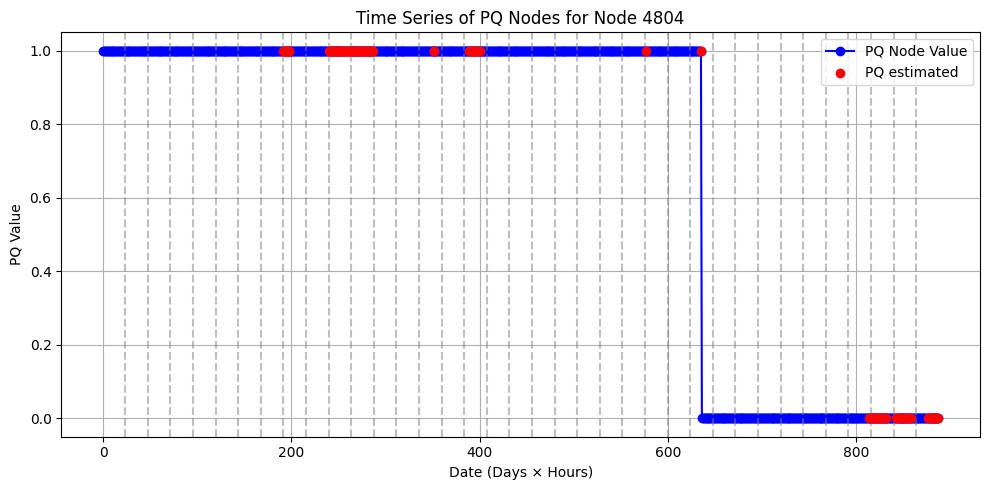
\includegraphics[width=0.7\textwidth]{picture/PQ_nodes.png}
    \caption{PQ\_nodes}
\label{fig:PQ_nodes}
\end{figure}

\begin{figure}[H]
    \centering
    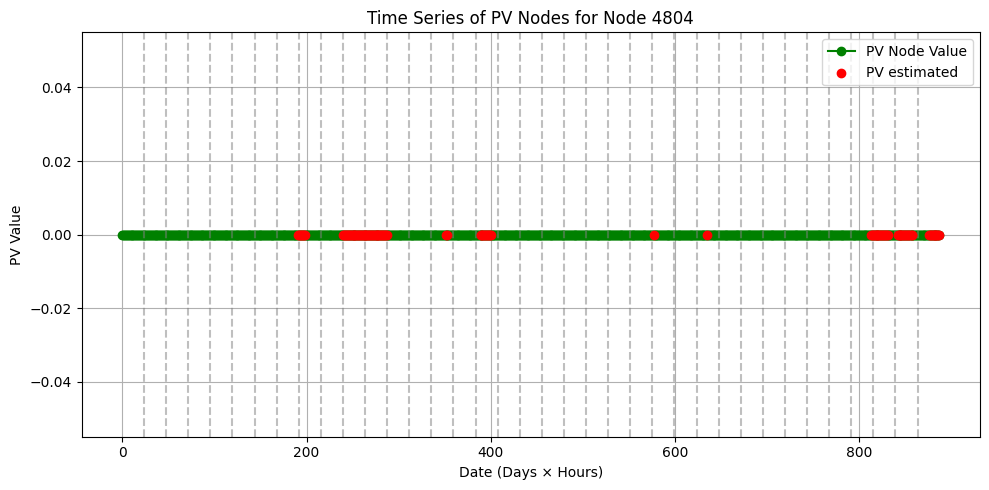
\includegraphics[width=0.7\textwidth]{picture/PV_nodes.png}
    \caption{PV\_nodes}
\label{fig:PV_nodes}
\end{figure}

\begin{figure}[H]
    \centering
    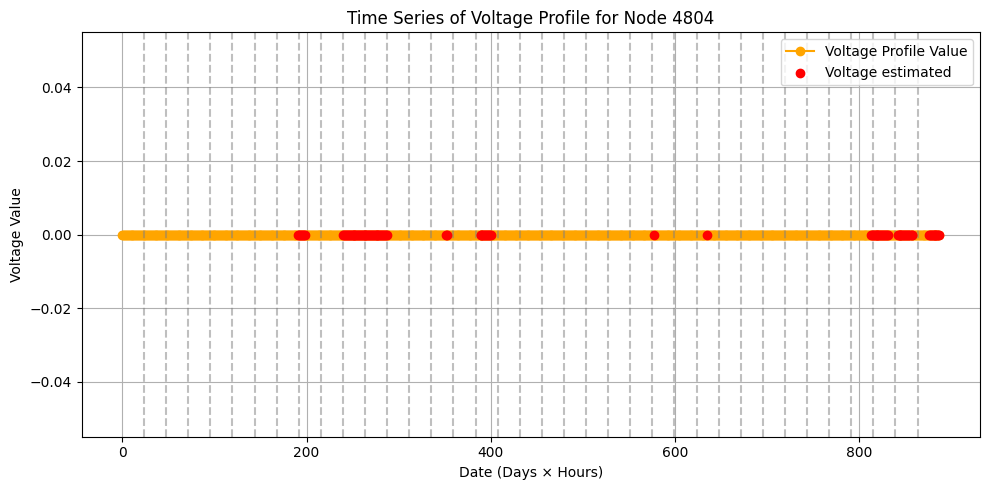
\includegraphics[width=0.7\textwidth]{picture/voltage_profile.png}
    \caption{voltage\_profile}
\label{fig:voltage_profile}
\end{figure}

As shown in Figure\ref{fig:PQ_nodes}, Figure\ref{fig:PV_nodes} and Figure\ref{fig:voltage_profile}, the respective data processing results are clearly visualized.

For the \emph{H matrix} field, we employ \emph{linear interpolation} to estimate the missing values in the H matrix. Specifically, we first sort the available data by their timestamps and, for each element of the matrix, apply linear interpolation using the existing time-series data. This method is then used to interpolate the matrix values at the missing (target) timestamps.

Linear interpolation provides a straightforward and efficient estimation approach. It is particularly suitable for power system data where changes often follow relatively simple patterns between consecutive time points, thus yielding a reliable reconstruction of the underlying H properties with minimal computational complexity.

Figure~\ref{fig:Avg_Magnitude} illustrates the variation in the average magnitude of the H matrix over time. 

\begin{figure}[H]
    \centering
    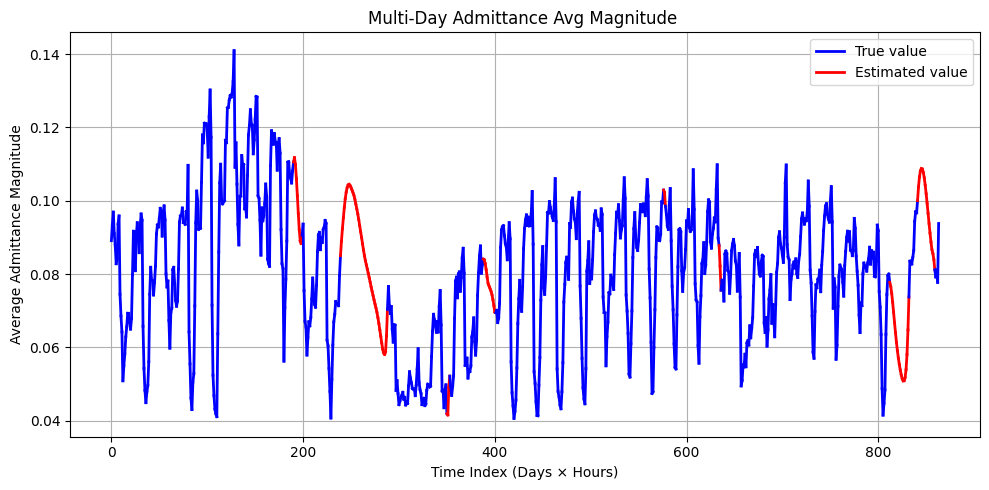
\includegraphics[width=0.7\textwidth]{picture/Avg_Magnitude.png}
    \caption{Avg\_Magnitude}
\label{fig:Avg_Magnitude}
\end{figure}

\section*{Data Records}

This dataset comprises \textbf{time-series weather data} and \textbf{power grid data}, collected at an \textbf{hourly resolution}. The dataset is structured into two key components:
\begin{itemize}
    \item \textbf{Weather Data}: Records environmental variables essential for energy-related applications.
    \item \textbf{Power Grid Data}: Captures grid topology, node attributes, power flow, and voltage information.
\end{itemize}
Each data file is stored in \textbf{NPZ format}, with the following naming convention: \texttt{YYYYMMDD\_HHMM.npz} (e.g., \texttt{20241020\_0000.npz} represents October 20, 2024, at 00:00).

\subsection*{Weather Data}
The weather dataset consists of six features, with each record representing an hourly snapshot of atmospheric conditions. Table \ref{tab:weather} summarizes these features.

\begin{table}[h]
    \centering
    \begin{tabular}{ll}
        \toprule
        \textbf{Feature} & \textbf{Description} \\
        \midrule
        \textbf{Date}  & Timestamp (YYYY-MM-DD HH:MM:SS) \\
        \textbf{hgv}   & Horizontal global irradiance (W/m²) \\
        \textbf{htv}   & Tilted surface irradiance (W/m²) \\
        \textbf{tempPv} & PV module temperature (°C) \\
        \textbf{windSpeed} & Wind speed (m/s) \\
        \textbf{windDir} & Wind direction (degrees) \\
        \bottomrule
    \end{tabular}
    \caption{Summary of Weather Data Features}
    \label{tab:weather}
\end{table}

These parameters are crucial for assessing \textbf{solar energy potential, weather-driven power fluctuations, and energy system performance}.

\subsection*{Power Grid Data}
The power grid dataset contains \textbf{structural and operational} information, enabling detailed analysis of electrical network behavior.

\subsubsection*{Node Attributes}
Each node in the power grid is classified into one of the following types:
\begin{itemize}
    \item \textbf{Load node}: Represents a consumption point within the grid.
    \item \textbf{Generator node}: Corresponds to a power generation source.
    \item \textbf{Balance node}: Ensures power equilibrium in the system.
\end{itemize}
The dataset also includes a \textbf{connectivity matrix}, representing the grid structure and interconnections between nodes.

\subsubsection*{Power and Voltage Features}
\begin{table}[h]
    \centering
    \begin{tabular}{ll}
        \toprule
        \textbf{Feature} & \textbf{Description} \\
        \midrule
        \textbf{P\_load} & Active power load at each node (MW) \\
        \textbf{Q\_load} & Reactive power load at each node (MVAR) \\
        \textbf{P\_gen} & Active power generation at each generator node (MW) \\
        \textbf{Q\_gen} & Reactive power generation at each generator node (MVAR) \\
        \textbf{Voltage Phase Angle (\(\theta\))} & Voltage phase angle at each node (degrees) \\
        \bottomrule
    \end{tabular}
    \caption{Summary of Power Grid Data Features}
    \label{tab:grid}
\end{table}

These parameters are vital for \textbf{grid stability analysis, load forecasting, and power distribution optimization}.

\subsection*{Data Storage \& Accessibility}
\begin{itemize}
    \item \textbf{Frequency}: Data is recorded hourly (\textbf{1-hour intervals}).
    \item \textbf{File Format}: NPZ (NumPy compressed archive).
    \item \textbf{File Naming Convention}: \texttt{YYYYMMDD\_HHMM.npz} (e.g., \texttt{20241020\_0000.npz}).
\end{itemize}
Each NPZ file contains structured arrays for easy data retrieval:

\begin{verbatim}
{
    "weather": np.array([...]),  # Shape: (N, 6) [hgv, htv, tempPv, windSpeed, windDir]
    "grid": {
        "connectivity": np.array([...]),  # Grid adjacency matrix or edge list
        "node_types": np.array([...]),  # Labels indicating node types
        "P_load": np.array([...]),  # Active power load
        "Q_load": np.array([...]),  # Reactive power load
        "P_gen": np.array([...]),  # Active power generation
        "Q_gen": np.array([...]),  # Reactive power generation
        "voltage_angle": np.array([...])  # Voltage phase angle
    }
}
\end{verbatim}

This dataset is well-suited for research in \textbf{renewable energy integration, power system optimization, and data-driven energy forecasting}.


\section*{Technical Validation}
\subsection*{Missing value imputation}
% 缺失值填补说明
\begin{figure}[htbp]
    \centering
    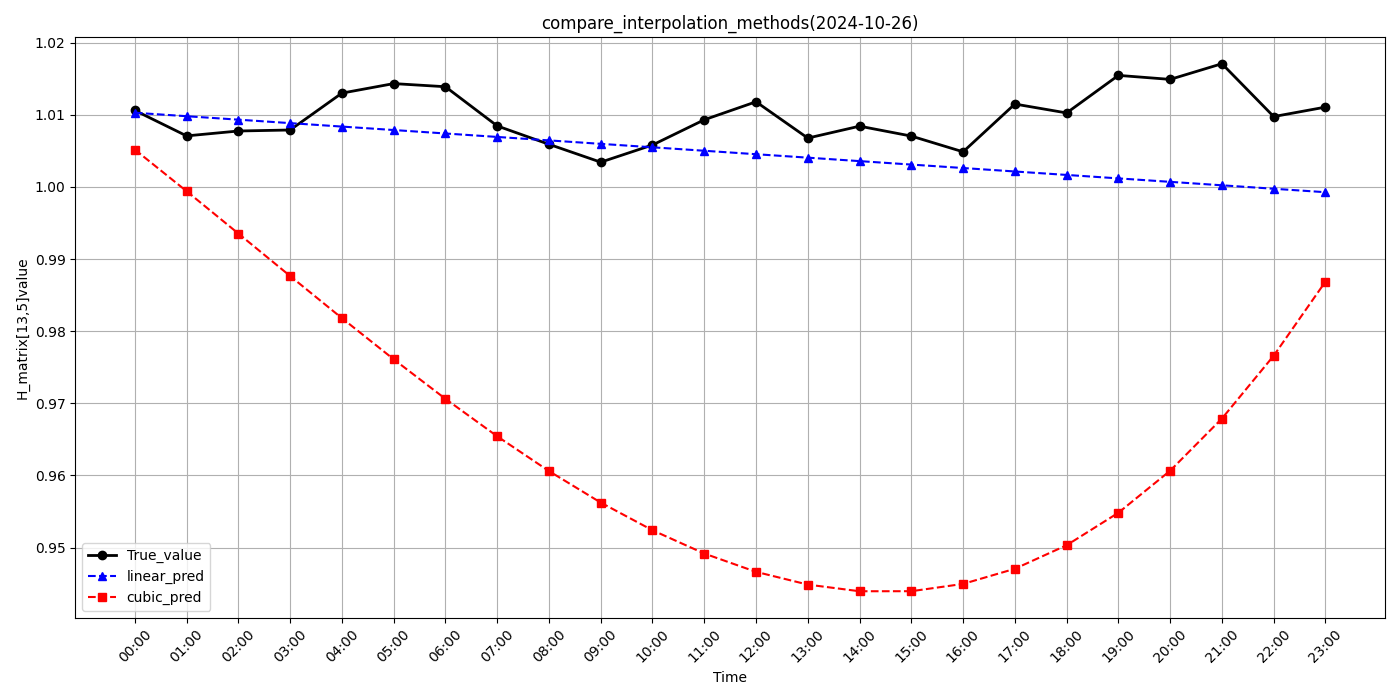
\includegraphics[width=0.85\textwidth]{picture/interpolation.png}
    \caption{Comparison of Linear and Cubic Spline Interpolation Methods}
    \label{fig:interpolation_comparison_en}
\end{figure}

\begin{table}[htbp]
    \centering
    
    \label{tab:interpolation_errors_en}
    \begin{tabular}{lccc}
        \toprule
        \textbf{Method} & \textbf{MSE} & \textbf{RMSE} & \textbf{MAE} \\
        \midrule
        Linear Interpolation & $5.6 \times 10^{-5}$ & $7.468 \times 10^{-3}$ & $5.770 \times 10^{-3}$ \\
        Cubic Spline Interpolation & $2.329 \times 10^{-3}$ & $4.826 \times 10^{-2}$ & $4.457 \times 10^{-2}$ \\
        \bottomrule
    \end{tabular}
    \caption{Error Metrics Comparison of Interpolation Methods}
\end{table}

For filling missing values in power system H matrices, we compared linear interpolation and cubic spline interpolation methods. As shown in Figure~\ref{fig:interpolation_comparison_en}, linear interpolation (blue line) demonstrated better performance than cubic spline interpolation (red line) on this dataset. The error metrics in Table~\ref{tab:interpolation_errors_en} clearly indicate that linear interpolation outperforms cubic spline interpolation in terms of MSE, RMSE, and MAE, with an MSE value approximately 1/41 of that of cubic spline interpolation. This may be due to the power system data exhibiting more linear temporal characteristics or containing certain noise patterns, which cubic spline interpolation tends to overfit. For this type of power system data, linear interpolation provides more accurate estimation results due to its simplicity and robustness.

\subsection*{Fault value diagnosis}
% 故障值诊断说明

\subsection*{Correlation analysis}
% 相关性分析说明
\subsection*{Load curve}
% 负荷曲线说明

\section*{Usage Notes}
% 使用说明

\section*{Acknowledgements}
% 致谢内容

% 请在此处插入引用,可以采用 BibTeX 或手动添加参考文献。
\bibliographystyle{unsrt}  % 可选 plain、alpha、abbrv 等格式
\bibliography{references}  % 请确保有一个名为 references.bib 的 BibTeX 数据库文件


\end{document}
